% \begin{document}
\chapter{Esercitazioni}

\section{Problemi e modelli}
\subsection{Problema dei data center}

\subsubsection{Testo}
Abbiamo $n$ server $1,\dots,n$, ogni server può lavorare in $m_{i\in\mathbb{N}}$ modalità operative diverse. Nella modalità $j\in\{1,\dots,m\}$, il server 1 riesce ad eseguire un numero di istruzioni..

\hspace{1.5cm}

\subsubsection{Svolgimento}

\textit{Variabili}:
\[
    \begin{aligned}
        x_{ij} &= \begin{cases}
            1 & \text{se il server $i$ è utilizzato in modalità $j\in\{1,\dots,m_i\}$} \\
            0 & \text{altrimenti}
        \end{cases}\\
        x_{ij}&\in \mathbb{N}, \quad \forall i\,\forall j
    \end{aligned}
\]
\textit{Vincoli}:
$\forall i\in \{1,\dots, n\},\quad\forall j\in\{1,\dots,m_{i}\}$ con $0\leq x_{ij}\leq 1$ si ha:
\[
    \begin{aligned}
        \forall i\in\{1,\dots,n\}\quad \sum_{j=1}^{m_i}x_{ij} &= 1\\
        \sum^n_{i=1}\sum^{m_i}_{j=1}x_{ij}s_{ij} &\geq k
    \end{aligned}
\]

\textit{funzione obbiettivo}

\[
    \min \sum^n_{i=1}\sum^{m_i}_{j=1}x_{ij}w_{ij}
\]

\subsection{Problema del docente di informatica}
\subsubsection{Testo}
Si hanno dei progetti ($t_1, t_2, \dots, t_n$), si hanno $m$ PC, dove ogni pc può compilare qualunque progetto in modalità sequenziale. Le prestazioni del PC sono identiche 

Vogliamo assegnare i progetti ai pc in modo da minimizzare il tempo complessivo parallelo di compilazione
\subsubsection{Svolgimento}
\textit{Variabili}:
\[
    \begin{aligned}
        x_{ij} &= \begin{cases}
            1 & \text{se il progetto $i$ è compilato al pc $j$} \\
            0 & \text{altrimenti}
        \end{cases}\\
        x_{ij}&\in \mathbb{N}, \quad \forall i\in \{1,\dots, n\}\,\forall j\in \{1,\dots, m\} \
    \end{aligned}
\]
\textit{Vincoli}:
\[
    \begin{aligned}
        \forall i\in\{1,\dots,n\}\quad \sum_{j=1}^{m}x_{ij} &= 1 \text{ (normale vincolo di semi-assegnamento!!)}\\
        \forall j\in\{1,\dots,m\}\quad y&\geq \sum^n_{i=1}x_{ij}t_i 
    \end{aligned}
\]
\textit{Funzione obbiettivo}:
\[
    \min (\underbrace{{\max_j \sum^n_{i=1}\underbrace{x_{ij}t_i}_{\text{tempo di compilazione del progetto $i$ al pc $j$}}}}_{\text{nonostante questa espressione matematica ha perfettamente senso, non è lineare!}})
\]

Funzione obbiettivo sbagliata! Pertanto prenderemo $y$ per "simulare" il massimo, di modo da rendere la funzione obbiettivo lineare:
\[
    \min y
\]

\subsection{Problema delle commesse}
\subsubsection{Testo}
Un'azienda deve decidere come impiegare i suoi $n$ dipendenti $1,\dots, n$.

L'azienda, nell'intervallo di tempo desiderato deve evadere $m$ commesse $1,\dots, m$

Ciascuna commessa $j$ deve essere svolta dal sottoinsieme $D_j\subseteq\{1,\dots, n\}$ dei dipendenti dall'azienda. 

Ogni commessa, se evasa darebbe luogo ad un ricavo pari a $r_j$ euro.

Ogni dipendente può lavorare ad una singola commessa nell'unità di tempo 

\subsubsection{Svolgimento}
Si consideri che questo è un Problema di selezione di sottoinsiemi, infatti:
$\quad N=\{1,\dots,n\}$ elementi/dipendenti

$F = \{F_1, \dots, F_m\} \quad \text{dove } F_j$ è la $j$-esima commessa

\[
    a_{ij}= \begin{cases}
        1 & \text{se} i\in F_j\\
        0 & \text{altrimenti}
    \end{cases}
\]

\textit{Variabili}:
\[
    \begin{aligned}
        x_j= \begin{cases}
            1 & \text{se la commessa $j$ è evasa}\\
            0 & \text{altrimenti}
        \end{cases}\\
        x_j\in\mathbb{N} \quad \red{y_j\in\mathbb{N}}
    \end{aligned}
\]

\textit{Vincoli}:
\[
    \begin{aligned}
        0\leq x_j\leq 1 \quad \forall j\in\{1,\dots,m\} \quad \red{0\leq y_j\leq 1}\\
        \forall i\in\{1,\dots,n\}\quad \sum^m_{j=1}a_{ij}x_j &\leq 1 \quad \red{y_j=1-x_j}
    \end{aligned}
\]
\textit{Funzione obbiettivo}:
\[
    \max \sum^m_{j=1}r_jx_j \red{-\sum^m_{j=1}y_ip_j}
\]

\subsection{Problema della minimizzazione del massimo}
\subsubsection{Testo}
Una ditta di costruzioni edilizie ha deciso di subappaltare $n$ diverse opere ad $n$ diversi artigiani. Ad ogni artigiano $i = 1,\dots , n$ chiede di fornire il costo preventivo $c_{ij}$ che richiede per effettuare l’opera $j$, per ogni $j = 1, \dots, n$. Si vuole assegnare un’opera a ciascun artigiano in modo che tutte le opere siano effettuate e il costo massimo dei subappalti assegnati sia minimizzato. Formulare il problema

\subsubsection{Svolgimento}
\textit{Variabili}:
\[
    x_{ij} = \begin{cases}
        1 & \text{se l'opera $j$ è assegnata all'artigiano $i$}\\
        0 & \text{altrimenti}
    \end{cases}
\]

\textit{Vincoli}:
\[
    \forall j \sum^n_{i=1}x_{ij}=1 \quad \forall i \sum_{j=1}^n x_{ij}=1 
\]
Inoltre: 
\[
    \forall i, j\; c_{ij}x_{ij}\leq M
\]
\textit{Funzione obbiettivo}:
\[
    \min M
\]

\subsection{Problema della massimizzazione del minimo}
\subsubsection{Testo}
Si provi ora a massimizzare il costo minimo dei subappalti assegnati
\subsubsection{Svolgimento}
\textit{Variabili}:
\[
    x_{ij} = \begin{cases}
        1 & \text{se l'opera $j$ è assegnata all'artigiano $i$}\\
        0 & \text{altrimenti}
    \end{cases}
\]
\textit{Vincoli}:
\[
    \forall j \sum^n_{i=1}x_{ij}=1 \quad \forall i \sum_{j=1}^n x_{ij}=1
\]
Inoltre:
\[
    \forall i, j\; c_{ij}x_{ij}\geq m
\]
\textit{Funzione obbiettivo}:
\[
    \max m
\]

\subsection{Esercizio valore assoluto}
\subsubsection{testo}
Formulare il problema $\min\{|3 - 4x| : |x| \leq 2\}$
\subsubsection{Svolgimento}
\textit{Vincoli}
\[
    x \leq 2 \quad -x\leq 2
\]
\textit{Funzione obbiettivo}
\[
    \min\{3-4x\} \quad \min\{3-4x\}
\]

\subsection{Esercizio 1.26}

\textit{Variabili}

$ x_1,x_2 = \text{quantita di V1,V2} $

$ y_1,y_2,y_3 = \text{quantita di N1, N2, N3} $

$ z = \text{totale degli oli aquistati} $

\textit{Vincoli}

$ 0 \leq x_1 + x_2 \leq 200 $

$ 0 \leq y_1 + y_2 + y_3 \leq 250 $

$ z 3 \leq d_1x_1 + d_2x_2 + d_3y_1 + d_4y_2 + d_5y_3 \leq z 6  $

$ z = x_1 + x_2 + y_1 + y_2 + y_3 $ Dobbiamo fare in modo che $ z $ sia effetivamente il valore che gli vogliamo dare

\textit{Funzione Obbiettivo}

\[
 max\ 150 z - (110 x_1 + 120 x_2 + 130 y_1 + 110 y_2 + 115 y_3)
\]

\subsection{Esercizio 1.27}

\textit{Variabili}

$ x_1, x_2, x_3 = \text{numero di dolci A,B o C} $

$ x_1,x_2, x_3 \in \mathbb{N} $

\textit{Vincoli}

$ x_1 + x_2 + x_3 \leq 10000 $

$ x_1 \leq 0.5 x_1 + 0.5 x_2 + 0.5 x_3 $

$ x_3 \leq 0.25 x_2 $

\textit{Funzione Obbiettivo}

\[
0.2 x_1 + 0.1 x_2 + 0.4 x_3
\]

\subsection{Esercizio 1.28}

\textit{Variabili}

$ x_1,x_2,x_3 = \text{numero di beni prodotti con $ P_1, P_2, P_3 $} \in \mathbb{N} $

\textit{Vincoli}

$ 2x_1 + x_2 + 3x_3 \leq 50 $

$ 4x_1 + 2x_2 + 3x_3 \leq 50$

$ 3x_1 + 4 x_2 + 2x_3 \leq 50 $

$ 15 x_1 + 18 x_2 + 10 x_3 \geq 200 $

\textit{Funzione Obbiettivo}
\[
min \quad 4x_1 + 2 x_2 + 3 x_3
\]

\subsection{Esercizio 1.29}

\textit{Variabili}

$ x_1, x_2, x_3, x_4,x_5, x_6 = \text{numero ostetriche nuove a turno} \in \mathbb{N} $

\textit{Vincoli}

$ x_1 \geq 70 $

$ x_1 + x_2 \geq 80 $

$ x_2 + x_3 \geq 50 $

$ x_3 + x_4 \geq 60 $

$ x_4 + x_5 \geq 40 $

$ x_5 + x_6 \geq 30 $

\textit{Funzione Obbiettivo}
\[
min \quad x_1 + x_2 + x_3 +x_4 +x_5 +x_6
\]

\subsection{Esercizio 1.31}

\textit{Variabili}

$ \forall i = 1,...,7 \quad x_i = \text{variabili ogiche che indicano il fatto che un certo abitante $ a_i $ sia o meno membro del consiglio} $

\textit{Vincoli}

$ \sum_{i=1}^{7} x_i = 4 $

$ \forall i = 1,...,4 \sum_{x \in C_i} x = 1  $

$  $

\subsection{Esercizio 1.32}

\textit{Variabili}

$ x_i = \text{variabili logiche che mi dicono se scelgo i} $

\textit{Funzione Obbiettivo}

\[
max \quad \sum_{i=1}^{n} x_ib_i
\]

\textit{Vincoli}

$ \sum_{i=1}^{n} x_i = 11 $

$ 1 \leq \sum_{i \in C} x_i \leq 5 $

$ 1 \leq \sum_{i \in P} x_i \leq 1 $

$ 1 \leq \sum_{i \in D} x_i \leq 6 $

$ 1 \leq \sum_{i \in A} x_i \leq 4 $

$ \forall i = 1,...,m. \quad 0 \leq \sum_{i \in L_i} x_i  \leq 1 $

\subsection{Esercizio 1.35}

\textit{Variabili}

$ x_{ik} = \text{variabile logica che dice se teniamo l'impianto i per il mercato k} $

$ y_i = \text{variabile logica che dice se l'impianto i rimane aperto} $


\textit{Funzione obbiettivo}

$ min \quad \sum_{k \in K} \sum_{i \in I \cup J} x_{ik} c_{ik} b_k $

\textit{Vincoli}

$ \forall k \in K. \quad \sum_{i \in I \cup J} x_{ik} = 1 $

$ \sum_{i \in I} x_{ik} \geq \frac{|I|}{2} $ non va bene! possiamo contare piu' volte lo stesso impianto che pero' funziona su diversi mercati -> variabili ausiliarie 

$ \forall i \in I \cup J.\quad y_i \leq \sum_{k \in K} x_{ik} $ se tutti 0, allora y 0
$ y_i \geq x_{ik} $ disgiunzione logica generalizzata a k elemetni

$2 \sum_{i \in I} y_i \geq |I| $

$2 \sum_{i \in J} y_i \geq |J| $

\subsection{Esercizio 1.7}
\subsubsection{Testo}
Un’azienda di trasporti ha bisogno di
acquistare n litri di carburante ogni mese. Affinch´e gli autoveicoli funzionino a dovere, occorre
che il numero di ottani del carburante utilizzato sia almeno k. L’azienda acquista il suo
carburante da due fornitori A e B, che vendono carburante da kA e kB ottani, rispettivamente.
Sia A che B applicano un prezzo al litro piuttosto alto (pA e pB, rispettivamente) per i primi
s litri di carburante acquistati dall’azienda (ogni mese). Se il numero di litri acquistati ogni
mese supera s, i due fornitori applicano invece un prezzo al litro pi`u basso (ossia bA e bB,
rispettivamente), ma solo ai litri eccedenti s. Si formuli in PL il problema di determinare da
chi acquistare il carburante necessario ogni mese in modo da minimizzare il costo complessivo e
da rispettare il requisito sugli ottani.
\textit{Variabili}

\[
\begin{aligned}
    x_i &= \text{"litri da acquistare di tipo i"}    \\
    y_i &=\begin{cases}
        1 & \text{se }x_i\geq s\\
        0 & \text{altrimenti}
    \end{cases}\\
    z_{i1} &= \begin{cases}
        x_i &\text{se} 0<x_i<s\\
        0 &\text{altrimenti}
    \end{cases}\\
    z_{i2} &= \begin{cases}
        x_i - s &\text{se } x_i \geq s\\
        0 &\text{altrimenti}
    \end{cases}
    \end{aligned}
\]

\textit{Vincoli}

\[
    \begin{aligned}
        x_A + x_B &= n\\
        \frac{k_A \cdot x_A + k_b \cdot x_b}{n} &\geq k\\
        0 \leq z_i1 &\leq ()\\
    \end{aligned}
\]

\textit{Funzione Obbiettivo}
\[
    \min \sum_{i\in \{A,B\}} z_{i1}p_i + z_{i2}b_i + s p_1 y_i
\]

\subsection{Esercizio 1.6}
\subsubsection{Testo}
Una radio privata deve fare arrivare il suo segnale in una città che si trova al di là di una catena montuosa rispetto alla città da cui trasmette. Per fare ciò decide di installare \( n \) ripetitori sulla cima di altrettante colline, ciascuna delle quali si trova ad un'altitudine pari a \( a_i \). Il costo di costruzione di ogni ripetitore dipende dalla sua altezza: ogni metro costa \( c_i \). Occorre soddisfare solo un vincolo: il dislivello, in metri, tra la cima di un ripetitore e la cima del successivo non può superare una soglia pari a \( k \). Si formuli, in PL, il problema di decidere le altezze dei ripetitori in modo che il relativo costo sia minimo.

\subsubsection{Svolgimento}

\textit{Variabili}
\[
    \begin{aligned}
        x_i &= \text{"altezza del ripetitore i"}    \\
    \end{aligned}
\]



\textit{Vincoli}

\[
    \begin{aligned}
        \forall i\in[1\dots (n-1)] \quad x_{i+1} + a_{i+1} - x_{i} - a_{i} \leq k\\
        \forall i\in[1\dots (n-1)] \quad - x_{i+1} - a_{i+1} + x_{i} + a_{i} \leq k\\
    \end{aligned}
\]
\textit{Funzione Obbiettivo}

\[
    \min \sum_{i=1}^{n} c_i x_i
\]

\subsection{Esercizio 1.4 - Problema di Manutenzione degli Aerei}
\subsubsection{Testo}
Una compagnia aerea dispone di \( n \) aerei \( 1, \ldots, n \), e deve decidere in quale aeroporto, tra gli \( m \) in cui opera, svolgere le operazioni di manutenzione di ciascun aereo. Ogni aereo \( i \) è normalmente basato sull'aeroporto \( a_i \in \{1, \ldots, m\} \). Svolgere le operazioni di manutenzione di un aereo presso l'aeroporto \( j \) costa \( c_j \) euro. Se le operazioni di manutenzione si svolgono in un aeroporto diverso da quello in cui ogni aereo è basato, occorre poi sostenere un costo fisso pari a \( s \). Si formuli in PLI il problema di minimizzare i costi complessivi di manutenzione

\subsubsection{Svolgimento}

Bho, non ho capito, magari chiedere al prof


\subsection{Esercizio 1.3}
\subsubsection{Testo}
Una compagnia deve affittare dei computer per soddisfare il lavoro dei prossimi quattro mesi.

\begin{table}[h!]
\centering
\begin{tabular}{|c|c|c|c|c|}
\hline
Mese & Gennaio & Febbraio & Marzo & Aprile \\
\hline
Requisito & 9 & 5 & 7 & 9 \\
\hline
\end{tabular}
\caption{Requisiti mensili di computer.}
\end{table}

Il costo dell'affitto dipende dalla lunghezza dell'affitto stesso.

\begin{table}[h!]
\centering
\begin{tabular}{|c|c|c|c|}
\hline
Lunghezza & 1 mese & 2 mesi & 3 mesi \\
\hline
Costo & 200 & 350 & 450 \\
\hline
\end{tabular}
\caption{Costo dell'affitto in base alla lunghezza.}
\end{table}

Si dia una formulazione in programmazione lineare intera per il problema di trovare un piano di affitto di minimo costo.
\section{Tutor}

\subsection{Esercizio 1.24}

NON SO DOVE SIA IL RESTO DELL'ESERCIZIO

\textit{Variabili}

$ x_{ij} = \text{viene usato l'oleodotto che collega il giacimento i alla raffineria j} $

$ y_{ij} = \text{l'oleodotto ij viene utilizzato} $ variabile logica

\textit{FO}

\textit{Vincoli}

$ \forall i.\ \sum_{j = 1}^{m} x_{ij} = p_i $

$ \forall j. \sum_{i=1}^{n} x_{ij} \leq r_j $

$ \forall i,j.\ x_{ij} \leq y_{ij} \cdot a_{ij} $

\subsection{Esercizio 1.33}

\textit{Dati}

$ n = \text{num camion} $

$ \forall i = 1,...,n: $

$ m_i = \text{kilometri massimi percorribili per il camion i} $

$ k_i = \text{limite di kilometri per polizza bassa} $

$ c_i = \text{costo polizza quando } m_i \leq k_i $

$ d_i = \text{polizza quando } m_i > k_i $

\textit{Variabili}

$ p_i = \text{kilometri percorsi dal camion i} $

$ b_i = \text{il camion i utilizza la polizza bassa} $ variabile logica

\textit{Vincoli}

$ \sum_{i=1}^{n} p_i \geq 2000000 $ (possiamo mettere $ \geq $ e non $ = $ dato che minimizzando il valore ottimale sara' quello piu' basso)

$ m_i \leq b_i k_i + (1-b_i) m_i $

$ m_i > (1-b_i) k_i $

\textit{FO}
\[
  min \{\sum_{i=1}^{n} b_i c_i + (1-b_i) d_i \}
\]

\section{Esercitazioni reti di flusso con Luca}

\subsection{Ex 1}

\subsubsection{Testo}
Si risolva, tramite l’algoritmo di Edmonds e Karp il seguente problema di flusso massimo. Si determini altres`ı un taglio di capacit`a minima
\begin{center}
  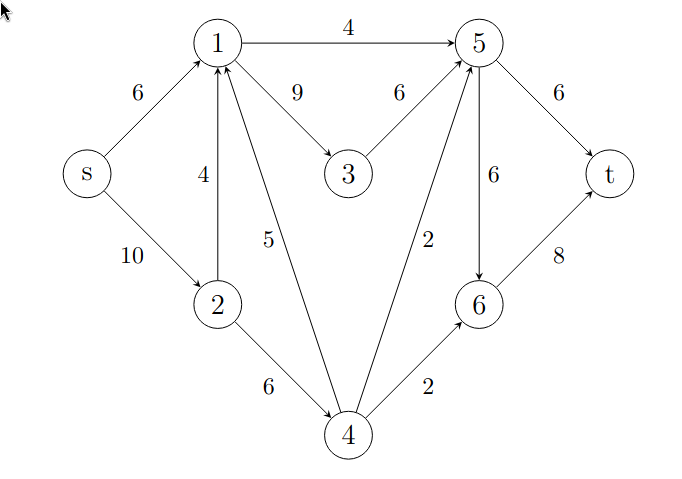
\includegraphics[width=0.5\textwidth]{img/2025-04-07-09-32-32.png}
\end{center}

\subsubsection{Soluzione}
In modo molto pratico, i passi sono:
\begin{enumerate}
\item Metti il flusso iniziale a 0 ovunque
\item Costruisci il grafo residuo (nota: il primo grafo residuo sara' uguale al grafo stesso)
\item Trova il cammino di lunghezza minima da s a t sul grafo residuo. Se non esiste, fine.
\item Identifica il valore minore fra gli archi del cammino. Poi, per tutti questi archi, aumentare o diminuire di questo valore il flusso dell'arco corrispondente sul grafo originale, in base a se l'arco residuo e' concorde o discorde all'arco associato.
\item Ritorna al punto 2
\end{enumerate}
Quindi, il meccanismo e':
\begin{enumerate}
\item Copia il grafo originale e trova su di esso un cammino, se non c'e' fine
\item Se c'e', calcola il valore minimo fra gli archi e aggiorna correttamente il valore dei flussi sul grafo originale
\item Col grafo OG aggiornato, costruire da questo un altro grafo residuo e ripetere da 2
\end{enumerate}

\nt{
  E' possibile risparmiarsi di etichettare i valori degli archi sui grafi residui, usando semplicemente le capacita' ed i flussi del grafo OG per trovare il valore minimo. Se l'arco e' concorde, il suo valore e' capienza - flusso, altrimenti e' semplicemente il flusso.
}

Facendo correttamente sti passi, arrivi a fine esecuzione con il valore del flusso $ v = 14 $.

\subsection{Ex 2}

\subsubsection{Testo}
Si risolva, tramite l’algoritmo di Goldberg-Tarjan il seguente problema MF.

\begin{center}
  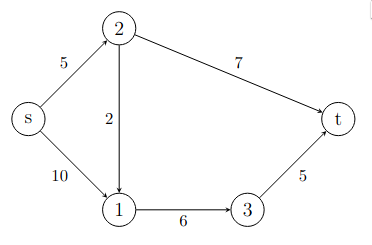
\includegraphics[width=0.5\textwidth]{img/2025-04-07-19-57-28.png}
\end{center}

Con Goldberg, si lavora a livello locale e non ci serve il grafo residuo. 

\subsection{Ex 3}

\subsubsection{Testo}
Si risolva il seguente problema MCF tramite l’algoritmo dei cammini minimi successivi.
\begin{center}
  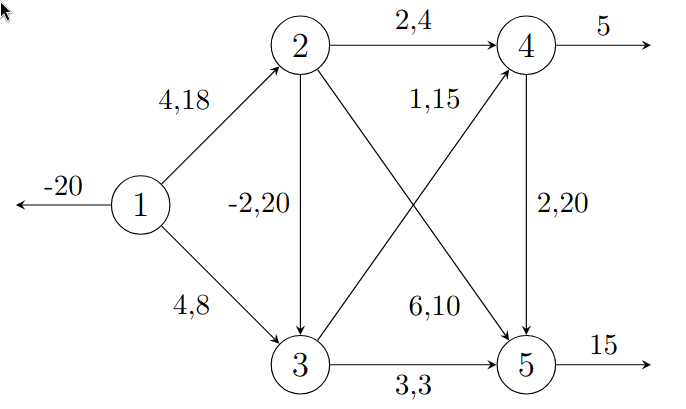
\includegraphics[width=0.5\textwidth]{img/2025-04-07-10-27-08.png}
\end{center}

\subsection{Ex 4}
\subsubsection{Testo}
Si risolva il precedente problema tramite l’algoritmo di cancellazione dei cicli.

% \end{document}
